\chapter{Beschreibung der verschiedenen Messungen und Ergbnisdarstellung}
\section{ISDN-Dienste}%Fragen 3, 10
\section{Verbindungsauf- und abbau}%Namen �berdenken

<<<<<<< HEAD
% \begin{figure}[htbp]
% \centering
% 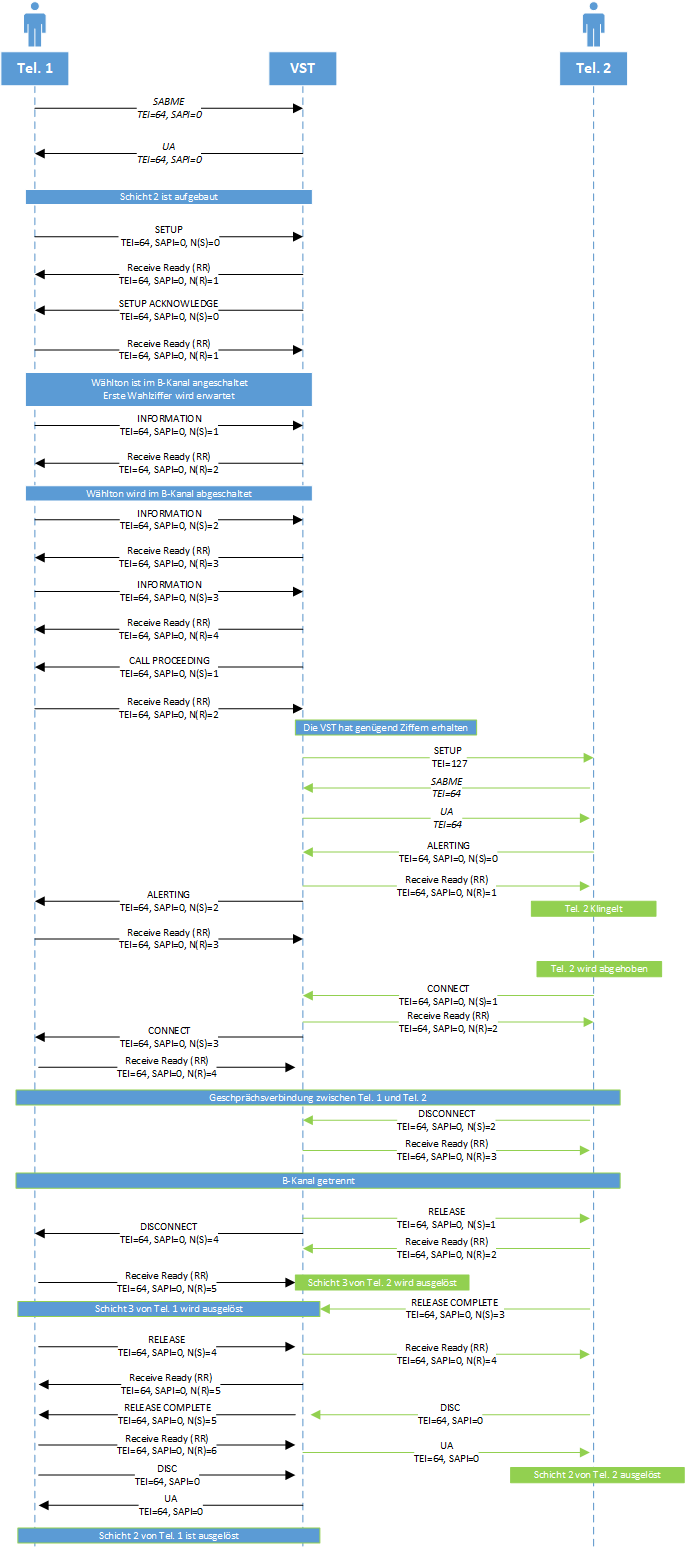
\includegraphics[keepaspectratio=true,scale=0.7]{Graphics/KRAUS.png}
% \caption{Verbindungsauf- und abbau}
% \label{fig:seq}
% \end{figure}

%\clearpage
=======
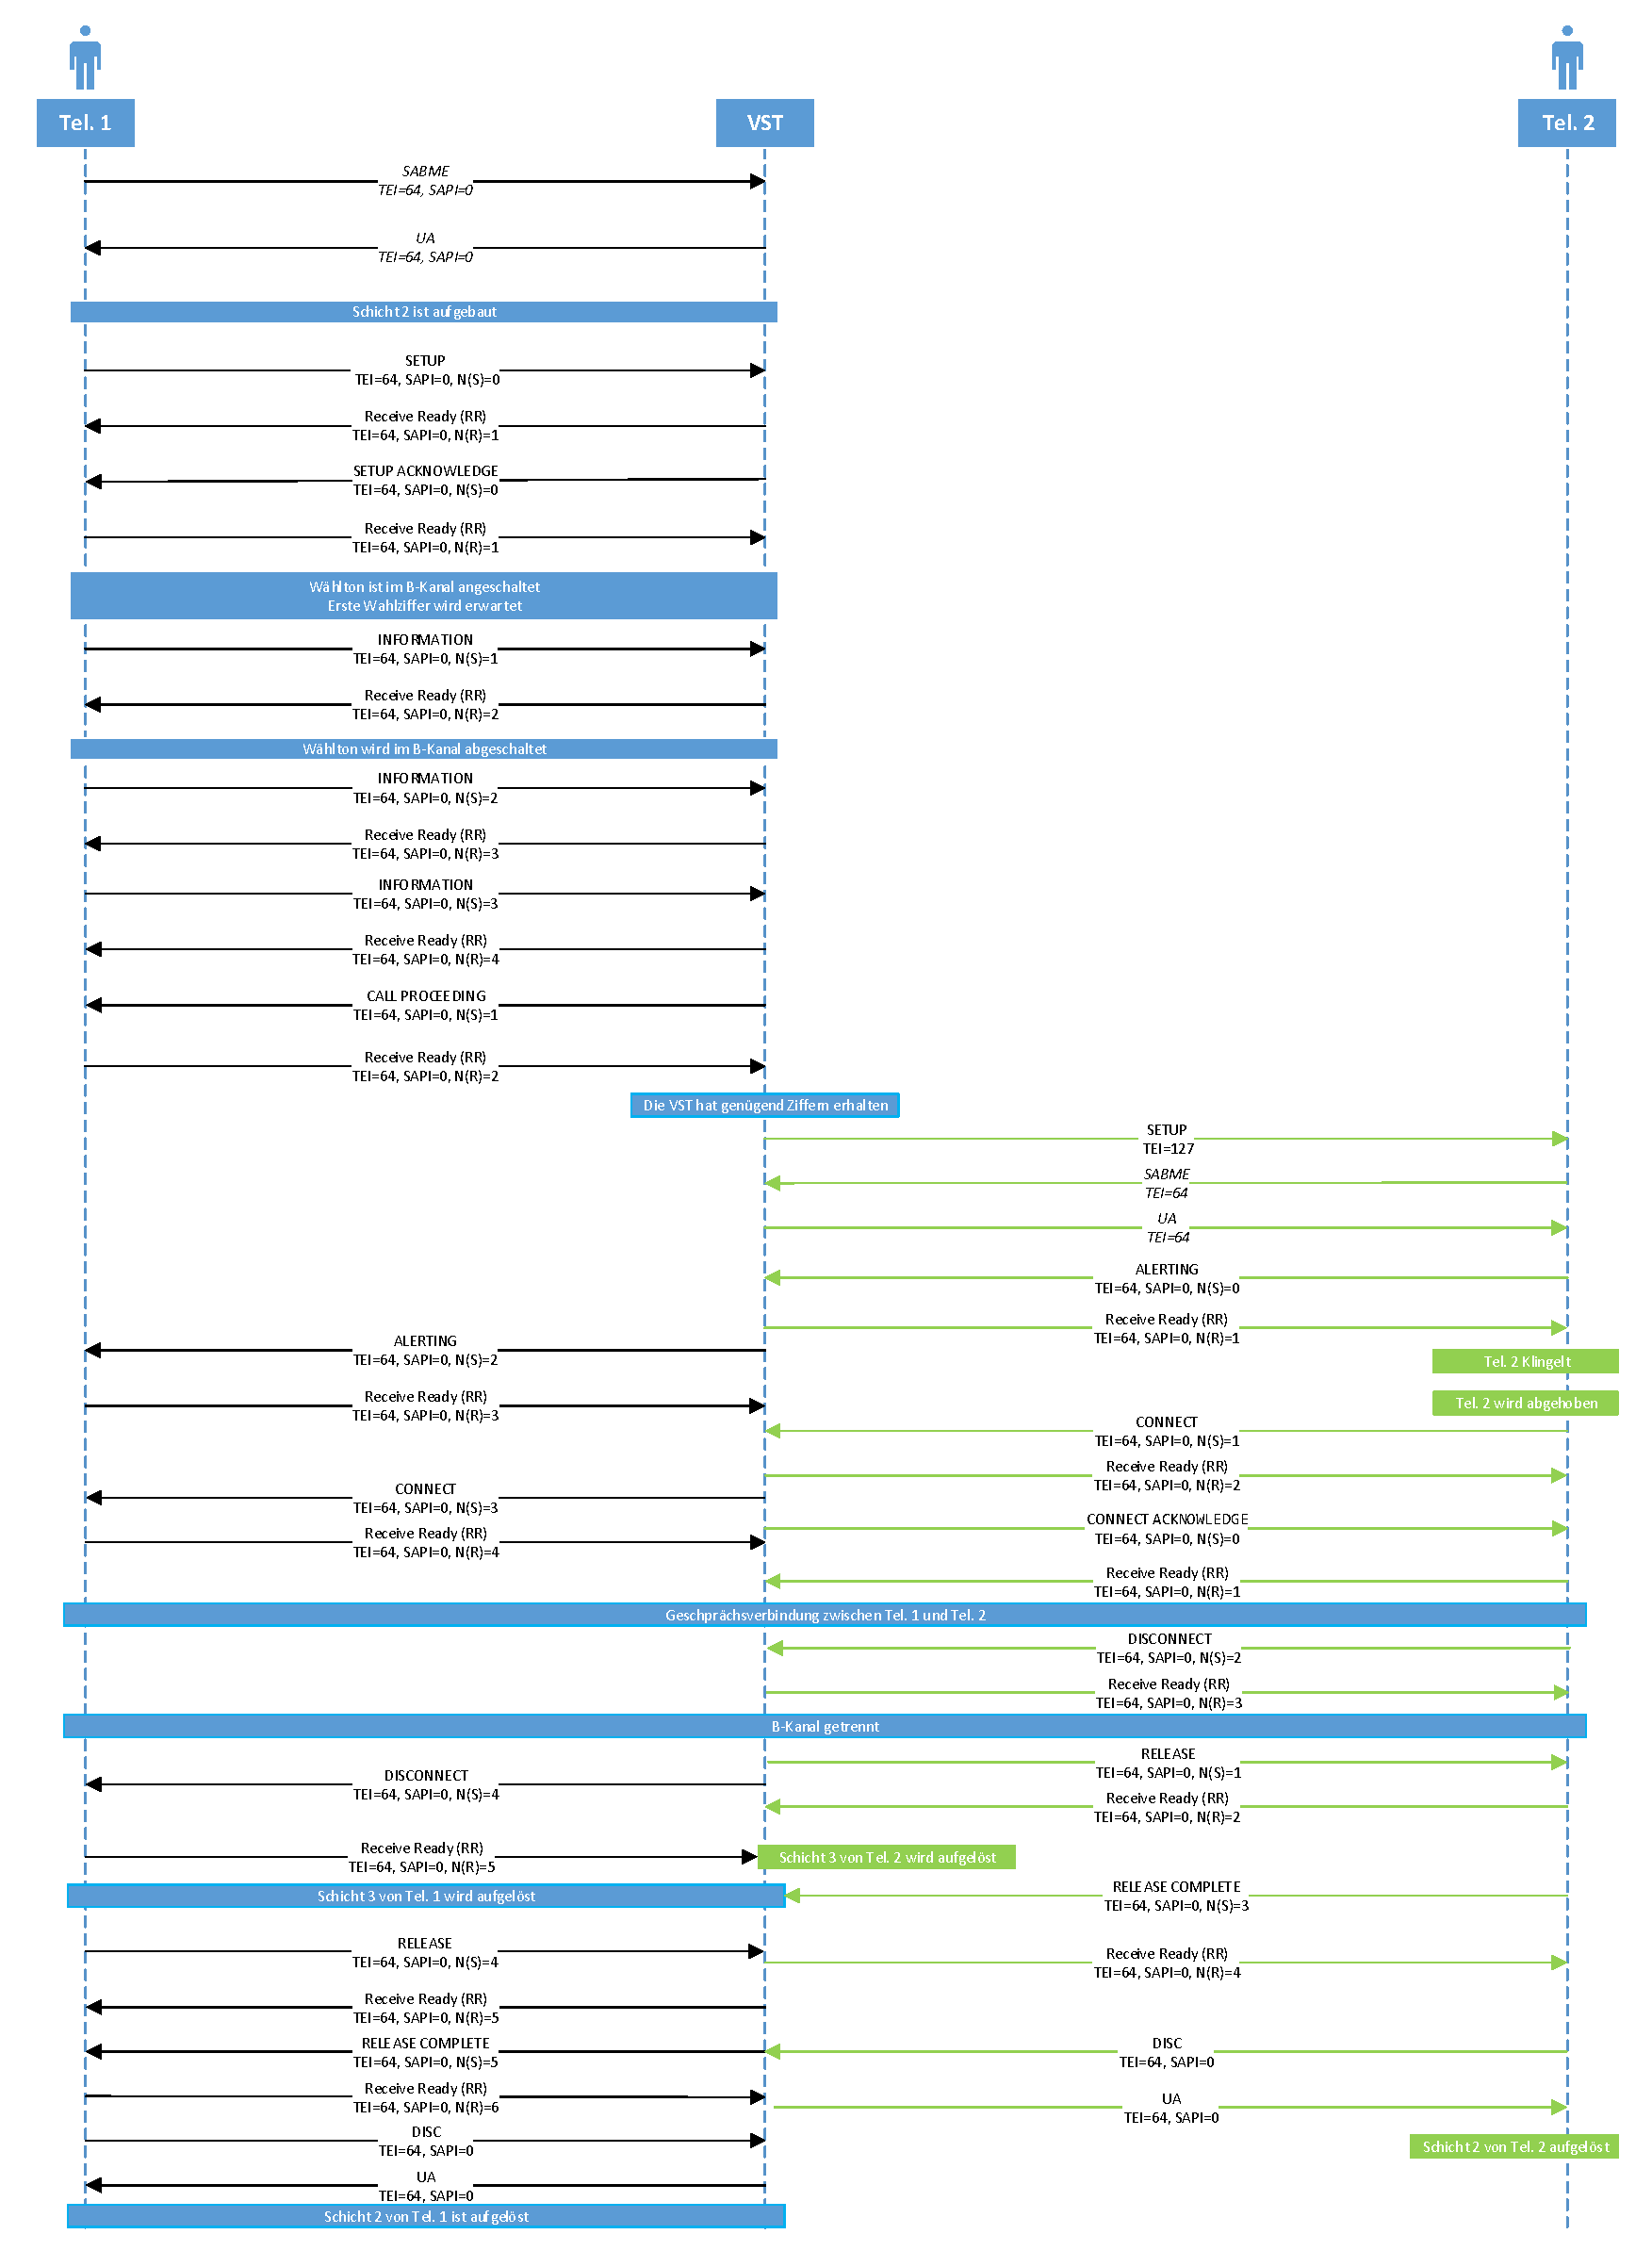
\includegraphics[width=\linewidth]{Graphics/KRAUS2}
\newline
\newline
Dieses Schaubild wurde anhand des Wireshark Mitschnittes erstellt und stellt den vollst�ndige Auf 
und Abbau der getestet Gespr�chsverbindung dar. Aus dem Wireshark mitschnitt konnte nur der linke 
teil der Nachrichten entnommen werden (Tel. 1 zu Vermittlungsstelle (VST) und umgekehrt). Der 
Rechte Teil der Nachrichten (VST und Tel. 2) hier gr�n dargestellt wurde zur Gesamtdarstellung
 hinzugef�gt. Zur Vervollst�ndigung wurde das Buch �Die Technik der Netze 1 von Gerd Siegmund� 
 (S. 357 -364) betrachtet.
\newline
\newline
Im ersten abschnitt findet der Aufbau einer Schicht 2 Verbindung statt. Dies erfolgt durch das 
Endger�t, da nur diese den eigene TEI kennt. Der Aufbau findet durch das senden der SABME Nachricht 
statt und wird durch die VST quittiert mit einer UA Nachricht. Dieser Austausch ist zeit�berwacht 
und dient dazu, alle Z�hler (Sende und Empfangsz�hler) zur�ckzusetzten. Wenn dieser Vorgang 
abgeschlossen ist, wurde die Schicht 2 aufgebaut und es k�nnen nummerierte I-Bl�cke ausgetauscht 
werden mit korrekter Z�hlernummer N(s) und N(R).
\newline
\newline
Nachdem die Schicht 2 aufgebaut wurde beginnt im Folgenden mit der SETUP Nachricht der Aufbau der 
Schicht 3, sowie die B-Kanal Zuweisung. Der Aufbau endet nach dem senden der Nachricht CONNECT 
ACKNOWLEDGE, diese dient der Best�tigung, dass der Anruf von Tel. 2 angenommen wurde und der 
Durchschaltung des B-Kanals im Netz. In unsrem Mitschnitt taucht diese jedoch nicht auf, da wir nur 
die anrufende Seite mitschneiden konnten und dort (wenn sie gesendet wird) von Tel. 1 zur VST 
gegangen w�re. In diesem Fall hat sie jedoch keine Bedeutung und kann entfallen. (Quelle Buch S.311)
\newline
\newline
Der Abbau der Schicht 3 wird durch die DISCONNECT Nachricht eingeleitet und ist mit der RELEASE 
COMPLETE Nachricht beendet. Danach erfolgt noch durch das aussenden der DISC Nachricht der Abbau 
der Schicht 2 dies wird wieder durch eine UA Nachricht quittiert.
%TODO Quelle
>>>>>>> branch 'master' of https://github.com/giraffenkaro/Praktikum.git
%auf die Schichten eingehen, vlt \subsection{Auf- und Abbau der Schichten}
%Fragen 2, 6, 11

\section{Adressierung der Endger�te}\label{tei}
Im Adressfeld des HDLC-Protokolls befindet sich der \ac{TEI}. Jedem Endger�t ist
ein solcher Identifier zugeordnet um eine logische Verbindung zwischen
Vermittlungsstelle und Endger�t sicherzustellen. Der TEI kennzeichnet die
Schicht-2-Adresse f�r das ISDN-Ger�t.\\%TODO Quelle: Net_IT, s.325
Der TEI-Wert kann entweder durch manuelle Einstellung am Ger�t hinterlegt werden
oder von der Vermittlungsstelle zugeteilt werden (TEI-Vergabe). In diesem
Versuch stellt das Endger�t zuerst eine Identity Request, worauf die
Vermittlungsstelle bei Erfolg mit Identity Assigned antwortet. Die Vergabe
erfolgt mittels U-Frame.%TODO: mehr
Dem Ger�t wird der TEI 64 zugeteilt. Dies ist der erste von der
Vermittlungsstelle zu vergebende Wert. Die Adressen 1-63 k�nnen eingestellt
werden, 64-126 werden von der Vermittlungsstelle verteilt. TEI 127 stellt die
Broadcast-Adresse dar.
\newline
\ac{SAPI} bezeichnet ein weiteres Element des HDLC-Adressfeldes und kennzeichnet
den momentan verwendeten ISDN-Schicht-2-Dienst.%TODO Quelle: siehe oben,s.326
Bei der TEI-Vergabe ist der Wert des SAPI 63. Dem Protokoll zufolge bedeutet
dies ``Layer 2 management procedures''. Es handelt sich hier um die �bertragung
von paketvermittelten Daten.%TODO Qzelle identisch

%TODO Zeilennummerierung

\begin{lstlisting}

No.     Time                       Source                Destination           Protocol Info
     56 2018-04-16 16:30:58.999168 User                  Network               TEI      Identity Request

Frame 56 (8 bytes on wire, 8 bytes captured)
    Arrival Time: Apr 16, 2018 16:30:58.999168000
    [Time delta from previous captured frame: 2.003968000 seconds]
    [Time delta from previous displayed frame: 2.003968000 seconds]
    [Time since reference or first frame: 19639.640168000 seconds]
    Frame Number: 56
    Frame Length: 8 bytes
    Capture Length: 8 bytes
    [Frame is marked: False]
    [Protocols in frame: isdn:lapd:tei_management]
    Point-to-Point Direction: Sent (0)
ISDN
    Channel: D (0)
Link Access Procedure, Channel D (LAPD)
    [Direction: User->Network (0)]
    Address Field: 0xfcff
        1111 11.. .... .... = SAPI: Layer 2 management procedures (63)
        .... ..0. .... .... = C/R: 0
        .... ...0 .... .... = EA1: 0
        .... .... 1111 111. = TEI: 127
        .... .... .... ...1 = EA2: 1
    Control field: U, func=UI (0x03)
        000. 00.. = Command: Unnumbered Information (0x00)
        .... ..11 = Frame type: Unnumbered frame (0x03)
TEI Management Procedure, Channel D (LAPD)

No.     Time                       Source                Destination           Protocol Info
     57 2018-04-16 16:30:59.005200 Network               User                  TEI      Identity Assigned

Frame 57 (8 bytes on wire, 8 bytes captured)
    Arrival Time: Apr 16, 2018 16:30:59.005200000
    [Time delta from previous captured frame: 0.006032000 seconds]
    [Time delta from previous displayed frame: 0.006032000 seconds]
    [Time since reference or first frame: 19639.646200000 seconds]
    Frame Number: 57
    Frame Length: 8 bytes
    Capture Length: 8 bytes
    [Frame is marked: False]
    [Protocols in frame: isdn:lapd:tei_management]
    Point-to-Point Direction: Received (1)
ISDN
    Channel: D (0)
Link Access Procedure, Channel D (LAPD)
    [Direction: Network->User (1)]
    Address Field: 0xfeff
        1111 11.. .... .... = SAPI: Layer 2 management procedures (63)
        .... ..1. .... .... = C/R: 1
        .... ...0 .... .... = EA1: 0
        .... .... 1111 111. = TEI: 127
        .... .... .... ...1 = EA2: 1
    Control field: U, func=UI (0x03)
        000. 00.. = Command: Unnumbered Information (0x00)
        .... ..11 = Frame type: Unnumbered frame (0x03)
TEI Management Procedure, Channel D (LAPD)
\end{lstlisting}


\section{Kanalzuweisung}%Fragen 4, 7,
Der Basisanschluss verf�gt �ber zwei B-Kan�le (Nutzkan�le) und einen D-Kanal
(Steuerkanal). %ITU T I.241.1

\section{Rufnummer und Wahlm�glichkeit}%Frage 5, 8, 9, 12


\section{Nachrichtenelemente}%Elemente erl�tern, zuordnen

\begin{tabularx}{\textwidth}{ |X|X|X|X|X|X|X|X|X|X| }
  \hline
  Nachricht  &Aler \newline ting&Call Proc&Con-nect&DISC&In-fo&Re-lease&Rel.
  Comp.&Set-up&Setup Ack \\
  \hline 
  Bearer Capability  &&&&&&&& M &  \\
  \hline
  Cause &&&&&&&&&  \\
  \hline
  Channel Identification  &&&&&&&&&  \\
  \hline
  Process Indicator  &&&&&&&&&  \\
  \hline
  Display  &&&&&&&&&  \\
  \hline
  Date/Time  &&&&&&&&&  \\
  \hline
  Calling Party Number  &&&&&&&&&  \\
  \hline
  Calles Party Number  &&&&&&&&&  \\
  \hline
  Sending Complete  &&&&&&&&&  \\
  \hline
  Facility  &&&&&&&&&  \\
  \hline
  User to User Information  &&&&&&&&&  \\
  \hline
\end{tabularx}


\section{Inhalt einer SETUP-Nachricht}


\begin{tabularx}{\textwidth}{ |X|X|X|X| }
  \hline
  & Bit-Nr. & Hex Code & Beschreibung \\
  \hline 
  Schicht-2-Header  & 0111 1110  & 0xFE  & Start-Flag  \\
  \hline
  Schicht-3-Paketkopf  &&&  \\
  \hline
  1. Info Element  &&&  \\
  \hline
  2. Info-Element  &&&  \\
  \hline
  3. Info-Element  &&&  \\
  \hline
  4. Info-Element  &&&  \\
  \hline
  Schicht-2-Trailer  & 0111 1110  &  & Ende-Flag  \\
  \hline
\end{tabularx}

